\documentclass[12pt]{book}
\usepackage[utf8]{inputenc}
\usepackage{color,soul,CJK,epic,tikz,array}
\usepackage{amsmath,amsthm,amssymb}
\usepackage{graphicx}
\usepackage{float}
\usepackage{subfigure}
\setlength{\parindent}{0em}
\author{andersonwu2000}
\pagestyle{empty}
\thispagestyle{empty} 

\newcounter{sect}

\newcounter{block}[sect]
\newenvironment{tblock}[1]
{\refstepcounter{block}\theblock.sim\begin{minipage}[t]{\dimexpr\linewidth}#1\\}
{\end{minipage}\\}

\newenvironment{comm}
{\makebox[12pt][l]{$\bullet$}\begin{minipage}[t]{\dimexpr\linewidth}}
{\end{minipage}}

\begin{document}
\begin{CJK}{UTF8}{bsmi}

\hfill 2021/6/3 吳至堯 U10811023 \\

22.9. Show that $x$ is a generator of the cyclic group $(\mathbb{Z}_3[x]/\left\langle x^3+2x+1 \right\rangle)^*$. \\
$Solution$. Let $F=\mathbb{Z}_3[x]/\left\langle x^3+2x+1 \right\rangle$, \\
then $|F|=3^3=27$ and $|F^*|=27-1=26$. \\
Since $|F^*|=27-1=26$ and $F^*$ is cyclic under multiplication \\
$\quad\Rightarrow\quad$ the possible values of $|x|$ are 1, 2, 13, 26. \\
Since $x^1\ne1$ and $x^2\ne1$ \\
$\quad\Rightarrow\quad|x|\ne1$ and $2$. \\
Since $x^3+2x+1=0$ \\
$\quad\Rightarrow\quad x^3=-2x-1=x+2$. \\
Since $x^{13} = x(x^3)^4 = x(x+2)^4 = x^2(x+2)+2x(x+2)+2x^2+x = x^3+2x = 2 \ne 1$ \\
$\quad\Rightarrow\quad|x|\ne13$ and $|x|=26$. \\
Hence $x$ is a generator of the cyclic group $(\mathbb{Z}_3[x]/\left\langle x^3+2x+1 \right\rangle)^*$. \\

22.11. Suppose that $F$ is field of order 1024 and $F^*=\left\langle \alpha \right\rangle$. List the elements of each subfield of $F$. \\
$Solution$. The subfields of $F$ are \\
\begin{tabular}{l}
    $GF(2^1)  
    = \{0\} \cup \left\langle \alpha^{(1024-1)/(2-1)} \right\rangle
    = \{0\} \cup \left\langle \alpha^{1023} \right\rangle$, \\
    $GF(2^2)  = \{0\} \cup \left\langle \alpha^{341} \right\rangle$, \\
    $GF(2^5)  = \{0\} \cup \left\langle \alpha^{33} \right\rangle$, \\
    $GF(2^{10}) = \{0\} \cup \left\langle \alpha \right\rangle$ \\
\end{tabular}. \\

\clearpage

23.a. Let $\alpha$ and $\beta\ne0$ be constructible numbers, then so is $\alpha/\beta$. \\
$Solution$. Since $\frac{\alpha/\beta}{1}=\alpha/\beta$, $\alpha/\beta$ is a constructible number. \\
\begin{minipage}[t]{\dimexpr\linewidth-2em}
\begin{figure}[H] 
\centering 
\subfigure{
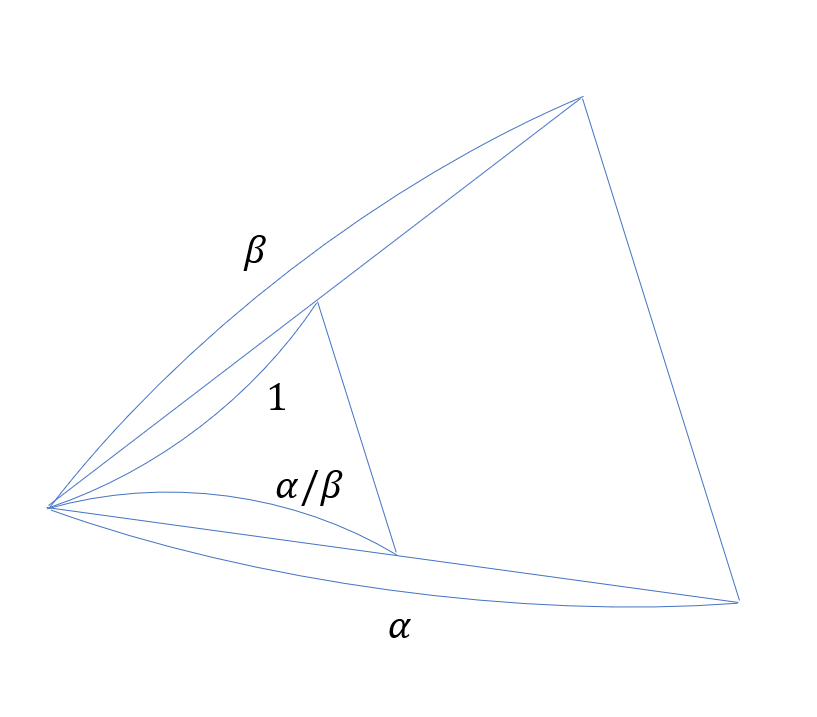
\includegraphics[width=0.7\textwidth]{HW(2)/ab.png}}
\end{figure}
\end{minipage}\\

23.b. Let $\alpha>0$ be constructible number, then so is $\sqrt{\alpha}$. \\
$Solution$. By Geometric mean theorem, $\sqrt{\alpha}$ is a constructible number. \\
\begin{minipage}[t]{\dimexpr\linewidth-2em}
\begin{figure}[H] 
\centering 
\subfigure{
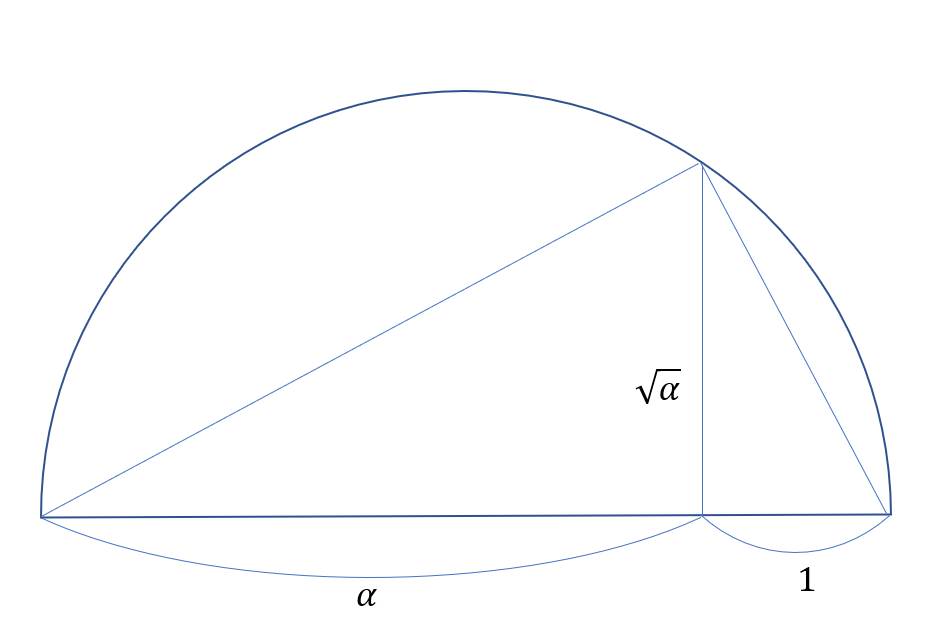
\includegraphics[width=0.7\textwidth]{HW(2)/sqrt(a).png}}
\end{figure}
\end{minipage}\\

\end{CJK}
\end{document}